%Big Game Hunter
\newcommand{\gameHunterDescription}{
\section{Big Game Hunter}
    Big Game Hunter Text\\
    See \nref{tlttree:gamehunter} for more information.
}

\newcommand{\gameHunterTree}{
    \newpage
    \subsection{Big Game Hunter Talent Tree}
    \label{tlttree:gamehunter}

    \textbf{Class Skills:} Athletics, Knowledge (Nature), Perception, Ranged, Stealth, Survival, 
    \newline

    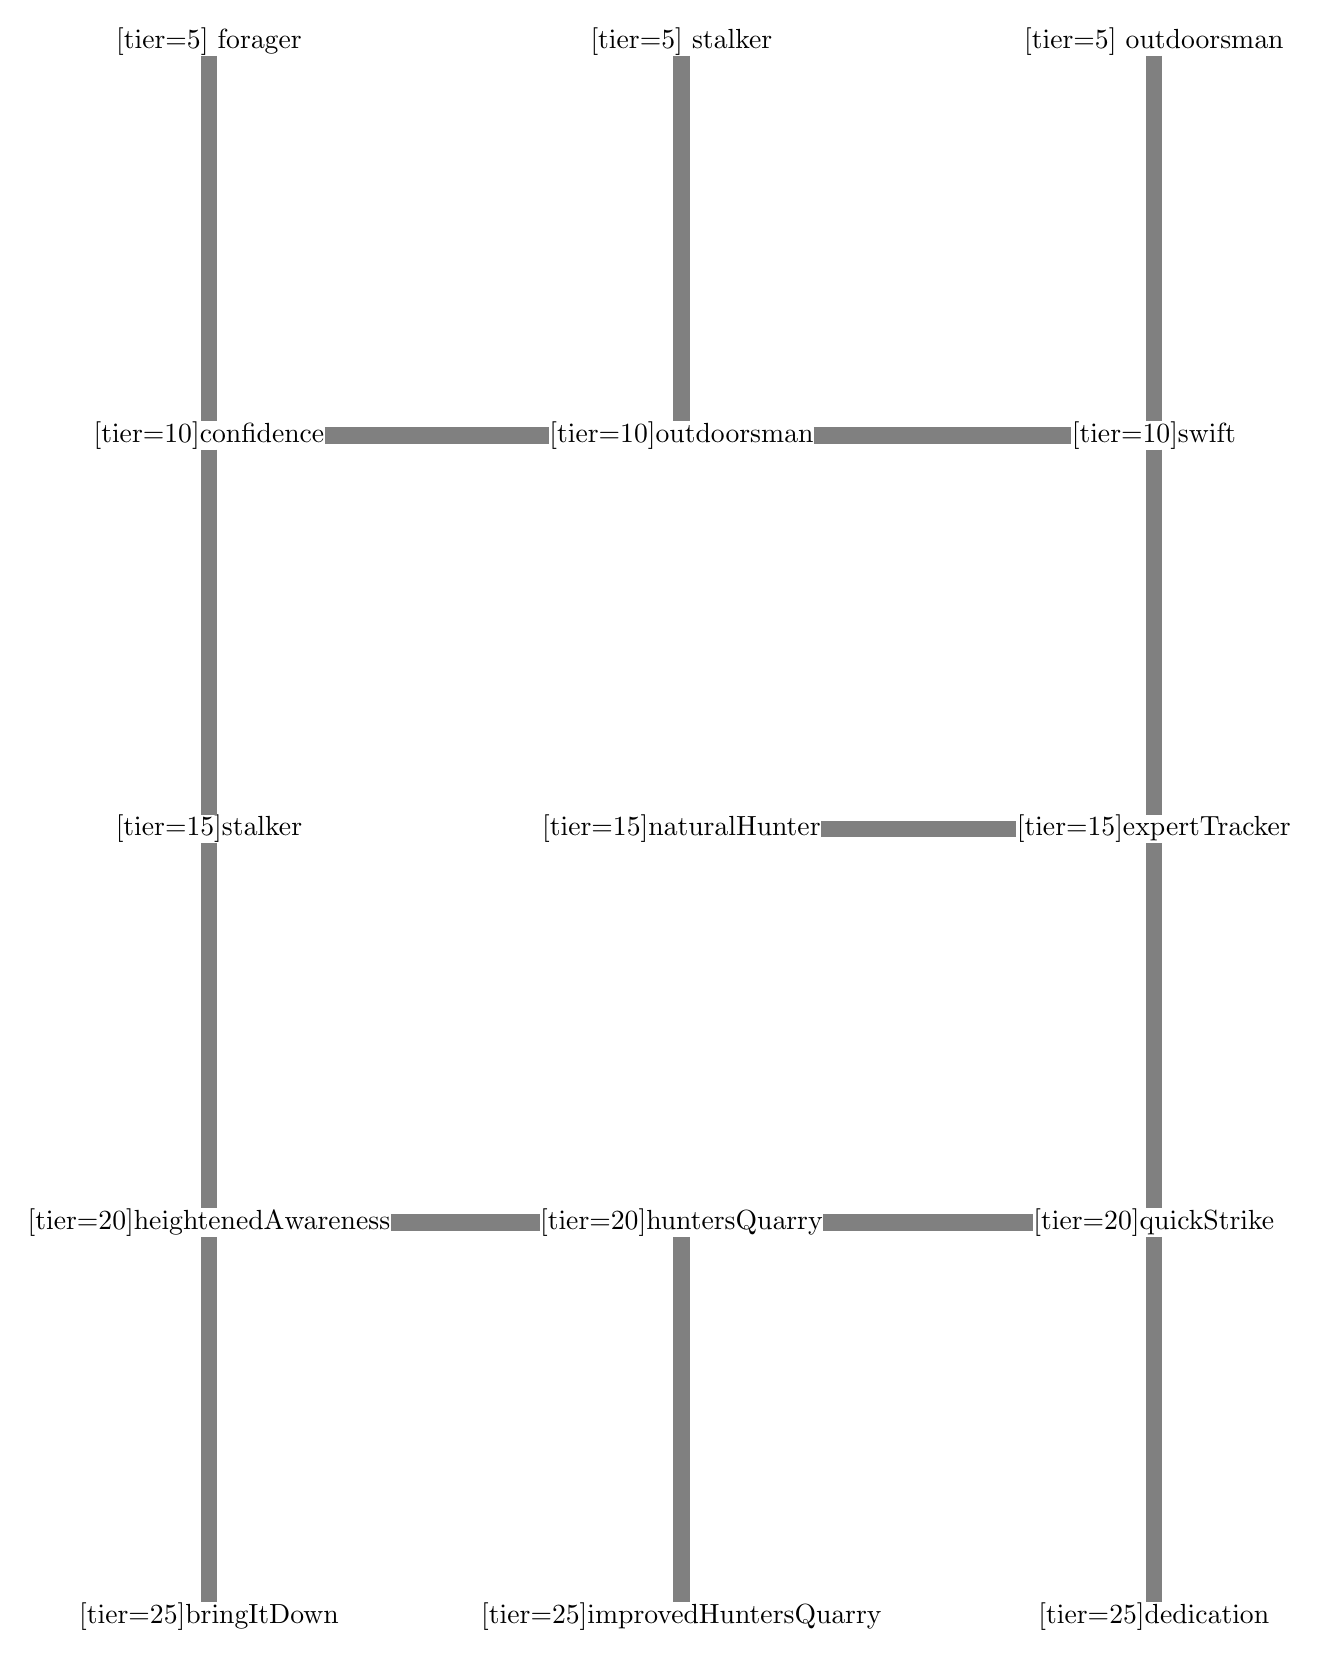
\begin{tikzpicture}
        \draw ( 0,  0) node(aa)[inner sep=0]{\TalentBox[tier=5] {forager}}
              ( 6,  0) node(ab)[inner sep=0]{\TalentBox[tier=5] {stalker}}
              (12,  0) node(ac)[inner sep=0]{\TalentBox[tier=5] {outdoorsman}}
              ( 0, -5) node(ba)[inner sep=0]{\TalentBox[tier=10]{confidence}}
              ( 6, -5) node(bb)[inner sep=0]{\TalentBox[tier=10]{outdoorsman}}
              (12, -5) node(bc)[inner sep=0]{\TalentBox[tier=10]{swift}}
              ( 0,-10) node(ca)[inner sep=0]{\TalentBox[tier=15]{stalker}}
              ( 6,-10) node(cb)[inner sep=0]{\TalentBox[tier=15]{naturalHunter}}
              (12,-10) node(cc)[inner sep=0]{\TalentBox[tier=15]{expertTracker}}
              ( 0,-15) node(da)[inner sep=0]{\TalentBox[tier=20]{heightenedAwareness}}
              ( 6,-15) node(db)[inner sep=0]{\TalentBox[tier=20]{huntersQuarry}}
              (12,-15) node(dc)[inner sep=0]{\TalentBox[tier=20]{quickStrike}}
              ( 0,-20) node(ea)[inner sep=0]{\TalentBox[tier=25]{bringItDown}}
              ( 6,-20) node(eb)[inner sep=0]{\TalentBox[tier=25]{improvedHuntersQuarry}}
              (12,-20) node(ec)[inner sep=0]{\TalentBox[tier=25]{dedication}}
        ;

        \tikzstyle{bar}=[gray,-,>=stealth, line width=6pt]

        \draw [bar] (aa) to (ba);
        \draw [bar] (ab) to (bb);
        \draw [bar] (ac) to (bc);

        \draw [bar] (ba) to (ca);
        \draw [bar] (bc) to (cc);

        \draw [bar] (ca) to (da);
        \draw [bar] (cc) to (dc);

        \draw [bar] (da) to (ea);
        \draw [bar] (db) to (eb);
        \draw [bar] (dc) to (ec);

        \draw [bar] (ba) to (bb);
        \draw [bar] (bb) to (bc);

        \draw [bar] (cb) to (cc);

        \draw [bar] (da) to (db);
        \draw [bar] (db) to (dc);

    \end{tikzpicture}
}
